\chapter{Theory}
\section{Furuta's Pendulum}
Rotational inverted pendulum or Furuta’s pendulum was firstly invented in 1992 at the Tokyo Institute of Technology by Katsuhisa Furuta as an example of a complex nonlinear oscillator in the sake of control algorithms testing in process control theory.
The pendulum composes of two main parts: motor-driven arm, which rotates in the horizontal plane and a pendulum, attached to that arm, which freely rotates in the vertical plane. The system is underactuated and extremely nonlinear due to the gravitational forces and the coupling arising from the Coriolis and centripetal forces. The schematic representation of the pendulum is shown in \ref{furuta}
\begin{figure}[h]
	\centering
	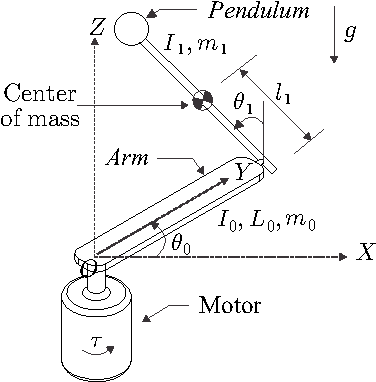
\includegraphics[width=.6\linewidth]{images/furuta}
	\caption{Furuta's Pendulum}
	\label{furuta}
\end{figure}
\newpage
The symbols in the figure indicate the following:
\begin{itemize}
	\item \textbf{$g$} - gravitational acceleration [\si{\metre\per\square\second}]
	\item \textbf{$m_0$} - mass of arm [\si{\kilogram}]
	\item \textbf{$m_1$} - mass of pendulum [\si{\kilogram}]
	\item \textbf{$L_0$} - length of arm [\si{\metre}]
	\item \textbf{$L_1$} - length of pendulum [\si{\metre}]
	\item \textbf{$l_1$} - location of the pendulums center of mass [\si{\metre}]
	\item \textbf{$I_0$} - moment of inertia of arm [\si{\kilogram\per\square\metre}]
	\item \textbf{$I_1$} - moment of inertia of pendulum [\si{\kilogram\per\square\metre}]
	\item \textbf{$\theta_0$} - arm angle [\si{\radian}]
	\item \textbf{$\theta_1$} - pendulum angle [\si{\radian}]
	\item \textbf{$\tau$} - motor torque [\si{\volt}]
\end{itemize}
\subsection{Mathematical Model of the Pendulum}
To design a predictive controller, the knowledge of the dynamic model of the process is necessary. For that purpose, we found the discrete-time state-space representation the most suitable.
To obtain the state representation of the process the state variables must be defined first:
\begin{equation}
	\begin{bmatrix}
	x_1 & x_2 & x_3 & x_4
	\end{bmatrix}^\intercal = 
	\begin{bmatrix}
	\theta_0 & \dot{\theta_0} & \theta_1 & \dot{\theta_1}
	\end{bmatrix}^\intercal
\end{equation}
And the control variable:
\begin{equation} u = \tau \end{equation}
The analytical model is based on the equations of motion derived from the Lagrange equations of the second kind, which represent the most commonly used method for establishing equations of motion of difficult mechanical systems. This method is applied for obtaining mathematical models of eg manipulators, with several degreases of freedom. Taking into account damping in the
form of friction, the resulting equations of motion of the
pendulum are 
\begin{subequations}
	\begin{align}
	\ddot{\theta}_0 &= \frac{\gamma(\epsilon\dot{\theta_0}^2+\rho)-\delta(\tau+\beta\dot{\theta_1}^2-\sigma\dot{\theta_0}\dot{\theta_1})}{\gamma^2-\alpha\delta}\\
	\ddot{\theta}_1 &= \frac{\gamma(\tau+\beta\dot{\theta_1}^2-\sigma\dot{\theta_0}\dot{\theta_1})-\alpha(\epsilon\dot{\theta_0}^2+\rho)}{\gamma^2-\alpha\delta}
	\end{align}
\end{subequations}
where
\begin{subequations}
	\begin{align}
	\alpha &= I_0+L_0^2m_1+l_1^2m_1\sin^2\theta_1\\
	\beta &= L_0m_1l_1\sin\theta_1 \\
	\gamma &= L_0m_1l_1\cos\theta_1\\
	\delta &= I_1+l_1^2m_1\\
	\epsilon &= l^2_1m_1\sin\theta_1\cos\theta_1\\
	\rho &= m_1gl_1\sin\theta_1\\
	\tau &= 2l^2_1m_1\sin\theta_1\cos\theta_1
	\end{align}
\end{subequations}
These equations are further utilized to establish the state
space model
\begin{subequations}
	\begin{align}
\dot{x_1} &= \dot{\theta_0} \\
\dot{x_2} &= \frac{\gamma(\epsilon\dot{\theta_0}^2+\rho)-\delta(\tau+\beta\dot{\theta_1}^2-\sigma\dot{\theta_0}\dot{\theta_1})}{\gamma^2-\alpha\delta}\\
\dot{x_3} &= \dot{\theta_1}\\
\dot{x_4} &= \frac{\gamma(\tau+\beta\dot{\theta_1}^2-\sigma\dot{\theta_0}\dot{\theta_1})-\alpha(\epsilon\dot{\theta_0}^2+\rho)}{\gamma^2-\alpha\delta}
	\end{align}
\end{subequations}

Now these non-linear differential equations we can write in the form of matrices:
\begin{equation}\label{nonlinmodel}
\begin{bmatrix}
\dot{x_1} \\ \dot{x_2} \\ \dot{x_3} \\ \dot{x_4}
\end{bmatrix} = \begin{bmatrix}
\dot{\theta_0}\\
\frac{\gamma(\epsilon\dot{\theta_0}^2+\rho)-\delta(\tau+\beta\dot{\theta_1}^2-\sigma\dot{\theta_0}\dot{\theta_1})}{\gamma^2-\alpha\delta}\\
\dot{\theta_1}\\
 \frac{\gamma(\tau+\beta\dot{\theta_1}^2-\sigma\dot{\theta_0}\dot{\theta_1})-\alpha(\epsilon\dot{\theta_0}^2+\rho)}{\gamma^2-\alpha\delta}
\end{bmatrix}
\end{equation}
As we can see the derivatives of the states are the functions of the current states and control input. And more importantly, those variables have nonlinear interactions within each dynamic equation. 
\begin{equation}\begin{bmatrix}
\dot{x_1} \\ \dot{x_2} \\ \dot{x_3} \\ \dot{x_4}
\end{bmatrix} = f(x,u) =\begin{bmatrix}f_1(x,u)\\f_2(x,u)\\f_3(x,u)\\f_4(x,u)\end{bmatrix} \end{equation}
So that’s our non-linear dynamic model of the process. But only the NMPC controller is able to operate with such a model.  So, to make that model suitable for LQR and MPC controller we can approximate that non-linear model by a linear model as follows:
\begin{equation}\dot{x} = Ax + Bu\end{equation}
And the constant matrices are derived as:
\begin{equation}
A = \begin{bmatrix}
\frac{\partial f_1(x,u)}{\partial x_1}&\frac{\partial f_1(x,u)}{\partial x_2}&\frac{\partial f_1(x,u)}{\partial x_3}&\frac{\partial f_1(x,u)}{\partial x_4}\\
\frac{\partial f_2(x,u)}{\partial x_1}&\frac{\partial f_2(x,u)}{\partial x_2}&\frac{\partial f_2(x,u)}{\partial x_3}&\frac{\partial f_2(x,u)}{\partial x_4}\\
\frac{\partial f_3(x,u)}{\partial x_1}&\frac{\partial f_3(x,u)}{\partial x_2}&\frac{\partial f_3(x,u)}{\partial x_3}&\frac{\partial f_3(x,u)}{\partial x_4}\\
\frac{\partial f_4(x,u)}{\partial x_1}&\frac{\partial f_4(x,u)}{\partial x_2}&\frac{\partial f_4(x,u)}{\partial x_3}&\frac{\partial f_4(x,u)}{\partial x_4}
\end{bmatrix}, \quad B = \begin{bmatrix}
\frac{\partial f_1(x,u)}{\partial u}\\\frac{\partial f_2(x,u)}{\partial u}\\\frac{\partial f_3(x,u)}{\partial u}\\\frac{\partial f_4(x,u)}{\partial u}
\end{bmatrix}
\end{equation}
And when we compute these derivatives, we obtain a linearized model in the form of state matrices
\begin{subequations}
	\begin{align}
		A &=\begin{bmatrix}0&1&0&0\\
				0&0&\frac{-gL_0l_1^2m_1^2}{(m_1L_0^2+I_0)(m_1l_1^2+I_1)-L_0^2l_1^2m_1^2}&0\\
				0&0&0&1\\
				0&0&\frac{gl_1m_1(m_1L_0^2+I_0)}{(m_1L_0^2+I_0)(m_1l_1^2+I_1)-L_0^2l_1^2m_1^2}&0
			\end{bmatrix}\\
		B &=	\begin{bmatrix}
				0\\ 
				\frac{m_1L_1^2+I_1}{(m_1L_0^2+I_0)(m_1l_1^2+I_1)-L_0^2l_1^2m_1^2}\\
				0\\
				\frac{-L_0l_1m_1}{(m_1L_0^2+I_0)(m_1l_1^2+I_1)-L_0^2l_1^2m_1^2}
			\end{bmatrix}\\
		C &= \begin{bmatrix}0&0&1&0\end{bmatrix}\\
		D &= 0
	\end{align}
\end{subequations}
Now those linearized equations of motion would be evaluated at two equilibrium positions: upright and downward. The reason is that at the downward position the system's output, which is the position of the pendulum, has a stable point at “$+\pi$” and “$-\pi$”, while at the upright position system has no stable point.
 
The model, obtained by linearization around the upright operation point, is used for fulfilling the main control objective, which is stabilizing the pendulum at the upright position. The second model is used to simulate process behavior during initial excitation by a Swing-up controller.
\section{Controller Synthesis}
In this section theory for the individual controllers is described. As we are aiming for swing-up control of the pendulum, several controllers should be designed. For the heuristic swing-up approach an energy shaping controller and a predictive controller. And for the optimal swing-up approach a nonlinear model predictive control strategy.
\subsection{Model Predictive Control}
MPC uses a model of the system to make predictions about the system’s future behavior. MPC solves an online optimization algorithm to find the optimal control action that drives the predicted output to the reference. MPC can handle MIMO systems that may have interactions between their inputs and outputs. It can also handle input and output constraints. MPC has preview capability; it can incorporate future reference information into the control problem to improve controller performance. Due to all these properties MPC provides the highest quality of control performance at the moment.
\subsubsection{MPC formulation}
The model predictive control requires the linear discrete-time state-space model of the process
\begin{subequations}\label{linmodel}
	\begin{align}	
	x(t+\Ts) = Ax(t) + Bu(t)\\
	y(t) = Cx(t) + Du(t)
	\end{align}
\end{subequations}
Thanks to the knowledge of that model, we can predict the evolution of states and outputs of the system.\\
Due to the setup of the controlled process, the MPC should be formulated to regulate the states of the system to the origin. And such MPC can be formulated as
\begin{subequations}
	\begin{align}
		\min_{u_0,...,u_{N-1}} &\sum_{k=0}^{N-1} \lrp{\left\| \ui{Q}{x}x_{t+k}\right\|_p+\left\|\ui{Q}{u}u_{t+k}\right\|_p}\\
	    \label{eq217b}s.t.\quad&x_{t+k+1} = Ax_{t+k} + Bu_{t+k}\quad  k \in \mathbb{N}_0^{N-1}\\
		&x_t = x(t)\\
		\label{cst_x}&x_{t+k}\in\mathcal{X}\qquad\qquad\qquad\qquad  k \in \mathbb{N}_0^{N-1}\\
		\label{cst_u}&u_{t+k}\in\mathcal{U}\qquad\qquad\qquad\qquad\,  k \in \mathbb{N}_0^{N-1}
	\end{align}
\end{subequations}
where $\mathcal{X}$ and $\mathcal{U}$ are polytopic state and input constraints respectively and defined as
\begin{subequations}
	\begin{align}
	\mathcal{X} &= \{\ui{H}{x}x\leq \ui{K}{x}\}\\
	\mathcal{U} &= \{\ui{H}{u}u\leq \ui{K}{u}\}
	\end{align}
\end{subequations}
Unfortunately, such formulation is inappropriate for quadratic programming solver, so it has to be reformulated in the form of a quadratic optimization problem.
\subsubsection{MPC as a QP optimisation problem}
The QP optimization problem has the following form
\begin{subequations}
	\begin{align}
	\min_{u_0,...,u_{N-1}} & z^\intercal Pz + 2Q^\intercal z + R\\
	\label{cst_qp}s.t.\quad&Hz\leq G\\
	&\ui{H}{eq}z = \ui{G}{eq}
	\end{align}
\end{subequations}
As the first step, the standard MPC cost function should be written in a vector form
\begin{equation}
	\min_{u_0,...,u_{N-1}} X^\intercal\ui{\tilde{Q}}{x}X + U^\intercal\ui{\tilde{Q}}{u}\,U\\
\end{equation}
where $X$ is a vector of predicted states, $U$ is an optimal trajectory of future control inputs and $\tilde{Q}_x$ and $\tilde{Q}_u$ are the matrices of original weight matrices.
\begin{equation}
	X = \begin{bmatrix}
	x_t\\x_{t+1}\\\vdots\\x_{t+N-1}
	\end{bmatrix}
\end{equation}
\begin{equation}
U = \begin{bmatrix}
u_t\\u_{t+1}\\\vdots\\u_{t+N-1}
\end{bmatrix}
\end{equation}
\begin{equation}
\tilde{Q}_x = \begin{bmatrix}
Q_x&0&\cdots&0\\
0&Q_x&\cdots&0\\
\vdots&\vdots&\ddots&\vdots\\
0&0&\cdots&Q_x
\end{bmatrix}
\end{equation}
\begin{equation}
\tilde{Q}_u = \begin{bmatrix}
Q_u&0&\cdots&0\\
0&Q_u&\cdots&0\\
\vdots&\vdots&\ddots&\vdots\\
0&0&\cdots&Q_u
\end{bmatrix}
\end{equation}
At the next step, the equality constrains (\ref{eq217b}) should be expressed in the vector form. We can achieve that by predicting the evolution of states over the whole prediction horizon.
\begin{equation}
\begin{split}
x_t &= x(t)\\
\hat{x}_{k+1} &= Ax_k + Bu_k\\
\hat{x}_{k+2} &= A\hat{x}_{k+1} + Bu_{k+1}\\
&= A^2x_k + ABu_k + Bu_{k+1}\\
\hat{x}_{k+3} &= A\hat{x}_{k+2} + Bu_{k+2}\\
&= A^3x_k + A^2Bu_k + ABu_{k+1} + Bu_{k+2}\\
&\vdots\\
\hat{x}_{k+N} &= A^Nx_k+\sum_{j=k}^{k+N-1}A^jBu_{k+N-j-1}
\end{split}
\end{equation}
Or, if we write these equations in a compact form, we obtain
\begin{equation}
	\begin{bmatrix}
	x_t\\\hat{x}_{t+1}\\ \hat{x}_{t+2}\\\vdots\\ \hat{x}_{t+N-1}
	\end{bmatrix} = 
	\begin{bmatrix}I\\A\\A^2\\ \vdots \\ A^{N-1}\end{bmatrix}x(t) + 
	\begin{bmatrix}
	0& 0&\cdots&0&0\\
	B&0&\cdots&0&0\\
	AB&B&\cdots&0&0\\
	\vdots&\vdots&\ddots&\vdots&\vdots\\
	A^{N-2}B&A^{N-3}B&\cdots&B&0\end{bmatrix}
	\begin{bmatrix}u_k\\u_{k+1}\\u_{k+2}\\\vdots\\u_{k+N-1}\end{bmatrix}
\end{equation}
Or in the short form
\begin{equation}\label{eq227}
	X = \tilde{A}x_t + \tilde{B}U
\end{equation}
At this point, we can substitute as $X$ in the cost function by (\ref{eq227}). Then we obtain the new objective function
\begin{equation}\label{eq228}
	\min_{u_0,...,u_{N-1}} (\tilde{A}x_t + \tilde{B}U)^\intercal\ui{\tilde{Q}}{x}(\tilde{A}x_t + \tilde{B}U) + U^\intercal\ui{\tilde{Q}}{u}\,U\\
\end{equation}
And when we expand and simplfie (\ref{eq228}), we obtain
\begin{equation}
	U^\intercal(\tilde{B}^\intercal\ui{\tilde{Q}}{x}\tilde{B} + \ui{\tilde{Q}}{u})U + 2x_t^\intercal\tilde{A}^\intercal\ui{\tilde{Q}}{x}\tilde{B}U + x_t^\intercal\tilde{A}\ui{\tilde{Q}}{x}\tilde{A}x_t
\end{equation}
Where we can cleary see matrices $P$, $Q$ and $R$, which occurs in a standart cost function for the quadratic optimization.
\begin{subequations}
	\begin{align}
		P &= \tilde{B}^\intercal\ui{\tilde{Q}}{x}\tilde{B} + \ui{\tilde{Q}}{u}\\
		Q &= (2x_t^\intercal\tilde{A}^\intercal\ui{\tilde{Q}}{x}\tilde{B}U)^\intercal\\
		R &= x_t^\intercal\tilde{A}\ui{\tilde{Q}}{x}\tilde{A}x_t
	\end{align}
\end{subequations}
Now only constrains remain. Constrains (\ref{cst_x}) and (\ref{cst_u}) must be reformulated as (\ref{cst_qp}). Those constrains we consider as a upper and lower bounds for the states and control inputs respectively
\begin{subequations}
	\begin{align}
		\ui{x}{min} &\leq x_k \leq \ui{x}{max} \quad k \in \mathbb{N}_0^{N-1}\\
		\ui{u}{min} &\leq u_k \leq \ui{u}{max} \quad k \in \mathbb{N}_0^{N-1}
	\end{align}
\end{subequations}
Now we split and vectorise those constrains
\begin{subequations}
\begin{align}
	X &\leq \ \; \, \ui{X}{max}\\
	-X &\leq -\ui{X}{min}\\
	U &\leq \ \; \, \ui{U}{max}\\
	-U &\leq -\ui{U}{min}
\end{align}
\end{subequations}
In the next step, we substitute $X$ in the states constrains by a (\ref{eq227}) and express $U$
\begin{subequations}
	\begin{align}
	\tilde{B}\,U &\leq \ \; \,\ui{X}{max} - \tilde{A}x_t\\
	-\tilde{B}\,U &\leq -\ui{X}{min} + \tilde{A}x_t\\
	U &\leq \ \; \,\ui{U}{max}\\
	-U &\leq -\ui{U}{min}
	\end{align}
\end{subequations}
Those constraints are in the standard form and by combining them, we obtain matrices of inequality constraints $H$ and $G$ for the quadratic programming problem
\begin{equation}
	H = \begin{bmatrix}
	\ \; \,\tilde{B}\\
	-\tilde{B}\\
	\ \ \, I\\
	-I\\
	\end{bmatrix}, \quad
	G = \begin{bmatrix}
	\ \; \,\ui{X}{max} - \tilde{A}x_t\\
	-\ui{X}{min} + \tilde{A}x_t\\
	\ \ \:\ui{U}{max}\\
	-\ui{U}{min}
	\end{bmatrix}
\end{equation}
At this point, as matrices $R$, $Q$, $R$, $H$ and $G$ are defined, we can implement MPC by using any quadratic programming solver.
\subsection{Energy Shaping Controller}
For the initial excitation of the system, we use the energy-based swing-up controller. The strategy with this controller is that we increase the amplitude of swings by increasing the energy of the system with every swing. The energy is added by controlling arms movements and depends on the actual energy of the pendulum. The actual energy of the pendulum can be calculated from the actual position of the pendulum and its velocity: 
\begin{equation}
E = \frac{m_1gl_1}{2}\lrp{\lrp{\frac{\dot{\theta_1}}{\omega_0}}^2+\cos\theta_1 - 1}
\end{equation}
Than the control law has following form:
\begin{equation}
	u = \ui{k}{v}E\,\mathrm{sign}\lrp{\dot{\theta_1}\cos\theta_1}
\end{equation}
Where element $\mathrm{sign}\lrp{\dot{\theta_1}\cos\theta_1}$ determines direction i which the force will be applied and $k_vE$ is the gain of the controller.
\newpage
\subsection{Nonlinear Model Predictive Control}
In general to predict bechavior of the system MPC uses a linear predictive model (\ref{linmodel}). Though the original dynamic model of Furuta pendulum is nonlinear (\ref{nonlinmodel}) and such linearised model is precise only in short range around linearisation point. And as the main task is to perform swing-up control of the pendulum with the stabilization at the upright position via using only one controller, another control strategy should be designed.
\subsubsection{Nonlinear Programming Formulation}
To design an NMPC strategy, a Nonlinear Programming (NLP) problem should be formulated
\begin{subequations}\label{NLP}
	\begin{align}
	\min_{u_0,...,u_{N-1}} &\sum_{k=0}^{N-1} (\left\| \ui{Q}{x}x_{t+k}\right\|_p+\left\|\ui{Q}{u}u_{t+k}\right\|_p)\\
	s.t.\quad&x_{t+k+1} = \phi(x_{t+k},u_{t+k})\quad k \in \mathbb{N}_0^{N-1}\\
	&x_t = x(t)\\
	&x_{t+k}\in\mathcal{X}\qquad\qquad\qquad\quad\!\: k \in \mathbb{N}_0^{N-1}\\
	&u_{t+k}\in\mathcal{U}\qquad\qquad\qquad\quad\, k \in \mathbb{N}_0^{N-1}
	\end{align}
\end{subequations}
where $\phi(x_{t+k},u_{t+k})$ is a numerical integration operator that solves the following initial value problem (IVP) and returns the solution at $t_{k+1}$.
\begin{equation}
0=\ui{f}{impl}\lrp{\dot{x}(t), x(t),u(t),t},\quad x(0)=x_k.
\end{equation}
To solve such nonlinearly constrained optimization problem Sequential Quadratic Programming (SQP) algorithm will be used.
\subsubsection{Sequential Quadratic Programming}
SQP is the most successful method for solving nonlinearly constrained optimization problems. The basic idea of SQP is to model 
NLP at a given iterative $x^i$ as a Quadratic Programming (QP) subproblem, then the solulion of that QP subproblem is used to construct  a new iterate $x^{i+1}$.  And hopefully at the some point will converge to a solution $x^{*}$. This subproblem is assumed to reflect the local properties of the original problem.\\
For instance at iteration \textit{i} problem (\ref{NLP}) is linearized and  the following quadratic programming (QP) problem constucted:
\begin{equation}\label{QP}
\begin{aligned}
\min_{\Delta \mathbf{x},\Delta \mathbf{u}} \quad & \sum_{k=0}^{N-1}( \frac{1}{2}
\begin{bmatrix}
\Delta x_k\\
\Delta u_k
\end{bmatrix}^\intercal \begin{bmatrix}
Q_k^i & S_k^i \\
S_k^{i^\top} & R_k^i
\end{bmatrix}
\begin{bmatrix}
\Delta x_k\\
\Delta u_k
\end{bmatrix} + \begin{bmatrix}
g_{x_k}^i\\
g_{u_k}^i
\end{bmatrix}^\intercal
\begin{bmatrix}
\Delta x_k\\
\Delta u_k
\end{bmatrix} ) \\
s.t. \quad & \Delta x_0=\hat{x}_0-x_0,\\
& \Delta x_{k+1}=A_{k}^i \Delta x_{k}+ B_{k}^i \Delta u_{k} +a_{k}^i, \,\forall k \in \{0,...,N-1\}\\
& \underline{x}_k - x_k^i\leq \Delta x_k\leq \overline{x}_k-x_k^i,\,\forall k \in \{1,...,N\}\\
& \underline{u}_k - u_k^i\leq \Delta u_k\leq\overline{u}_k-u_k^i,\,\forall k \in \{0,...,N-1\}\\
\end{aligned}
\end{equation}
where 
\begin{equation}
\begin{aligned}
&\Delta \mathbf{x}=\mathbf{x}-\mathbf{x}^i,\\
&\Delta \mathbf{u}=\mathbf{u}-\mathbf{u}^i
\end{aligned}
\end{equation}
and
\begin{equation}\label{QP data}
\begin{aligned}
&g_{x_k}^i = \frac{\partial d^i}{\partial x_k},\quad g_{u_k}^i = \frac{\partial d^i}{\partial u_k},\\
&A_k^i=\frac{\partial \phi_k}{\partial x_k}, \quad B_k^i=\frac{\partial \phi_k}{\partial u_k},\quad a_k^i = \phi(x_k^i,u_k^i)-x_{k+1}^i,\\
\end{aligned}
\end{equation}
Where outer objective function $d:\mathbb{R}^{n_y}\rightarrow \mathbb{R}$, is convex. The Hessian matrices $Q_k,S_k,R_k$ can be approximated by the Gauss-Newton (GN) or the Generalized-Gauss-Newton (GGN) method. By solving that QP the optimal primal solution $(\Delta \mathbf{x}^{i^*}, \Delta \mathbf{u}^{i^*})$ is obtained. That primal solution is used to update the solution of \eqref{NLP} by
\begin{subequations}
	\begin{align}
\mathbf{x}^{i+1} = \mathbf{x}^{i} + \alpha^i \Delta\mathbf{x}^{i^*}, \\ \mathbf{u}^{i+1} = \mathbf{u}^{i} + \alpha^i \Delta\mathbf{u}^{i^*},
\end{align}
\end{subequations}
where $\alpha^i$ is the step length determined by globalization strategies. 